\documentclass{beamer}
\usepackage[utf8]{inputenc}
\usepackage{graphicx}
\usepackage{biblatex}
\usepackage{caption}
\graphicspath{ {./img/} }

%https://tex.stackexchange.com/questions/112576/math-mode-in-tabular-without-having-to-use-everywhere
\usepackage{array}   % for \newcolumntype macro
\newcolumntype{C}{>{$}c<{$}} % math-mode version of "l" column type

\title{Second Literature Review and Epidemic Model}
\author{Nima Seyedtalebi}

\date{April 18, 2019}
\bibliography{final_project.bib}
\begin{document}
\begin{frame}
    \maketitle
\end{frame}

\begin{frame}{Literature Review Assignment: Papers}
\begin{itemize}
    \item \fullcite{Hethcote2000TheMO}
    \item \fullcite{Pastor_satorras2014}
    \item \fullcite{Budak2011LimitingTS}
    \item \fullcite{Tambuscio2018NetworkSI}
\end{itemize}
\end{frame}

\begin{frame}{"Epidemic Processes in Complex Networks"}
\begin{itemize}
    \item A broad survey that aims to collect relevant research across disciplines
    \item The most important content is introduced in the early parts of the paper
    \item Later parts are mostly applications and extensions
    \item The examples for SIR models helped us choose a formulation
    \item Provides several examples of using mean-field theory to derive approximations
\end{itemize}
\end{frame}

\begin{frame}{"The Mathematics of Infectious Diseases"}
\begin{itemize}
    \item Another survey paper, more focused on mathematics in epidemiology
    \item Provides thorough treatment of classical SIS and SIR formulations
    \item Presents new expressions to find $R_{0}$ for MSEIR and SEIR models
    \item Includes applications of models to real-world data: measles in Niger and pertussis in US
\end{itemize}    
\end{frame}

\begin{frame}{"Limiting the Spread of Misinformation in Social Networks"}
    \begin{itemize}
        \item Aims to solve the Eventual Influence Problem (EIP): where to start information diffusion process to minimize effect of competing process once both have finished spreading
        \item Their models extend the independent cascade model:
        \begin{itemize}
            \item Upon activation, node tries once to activate each neighbor
            \item If a node receives multiple activations in a single timestep, one campaign gets priority
        \end{itemize}
        \item Their algorithm works well even with missing information
        \item The independent cascade model inspired the way we will model transmission
    \end{itemize}
\end{frame}

\begin{frame}{"Network Segregation in a Model of Misinformation and Fact-checking"}
\begin{itemize}
    \item This paper was a follow-up to \fullcite{Tambuscio15}
    \item Motivating question: how does network segregation affect the spread of misinformation and fact-checking?
    \item Split network into two groups with relatively few interconnections: gullible and skeptic
    \item Each group has different values for gullibility parameter $\alpha$
    \item Segregation effects depend mostly on forgetting probability 
    \item Effects can go either way - increase believers or fact-checkers at equilibrium
\end{itemize}
\end{frame}

\begin{frame}{Another Brief Intro to Compartmental Models}
    \begin{itemize}
        \item Population is organized into compartments based on status
        \item Common ones include Susceptible (S), Exposed (E), Infective (I), Recovered (R), and Passively-Immune (M)
        \item Note that "infective" \textit{does not mean the same thing as} "infected"
        \item Transition between compartments is governed by some set of rules
        \item Mathematical formulations that describe these rules abound
        \item Choices,choices: continuous or discrete-time, deterministic or stochastic, track individuals or populations...
    \end{itemize}
\end{frame}

\begin{frame}{General SEIR Model}
\begin{columns}
\begin{column}{0.48\textwidth}
    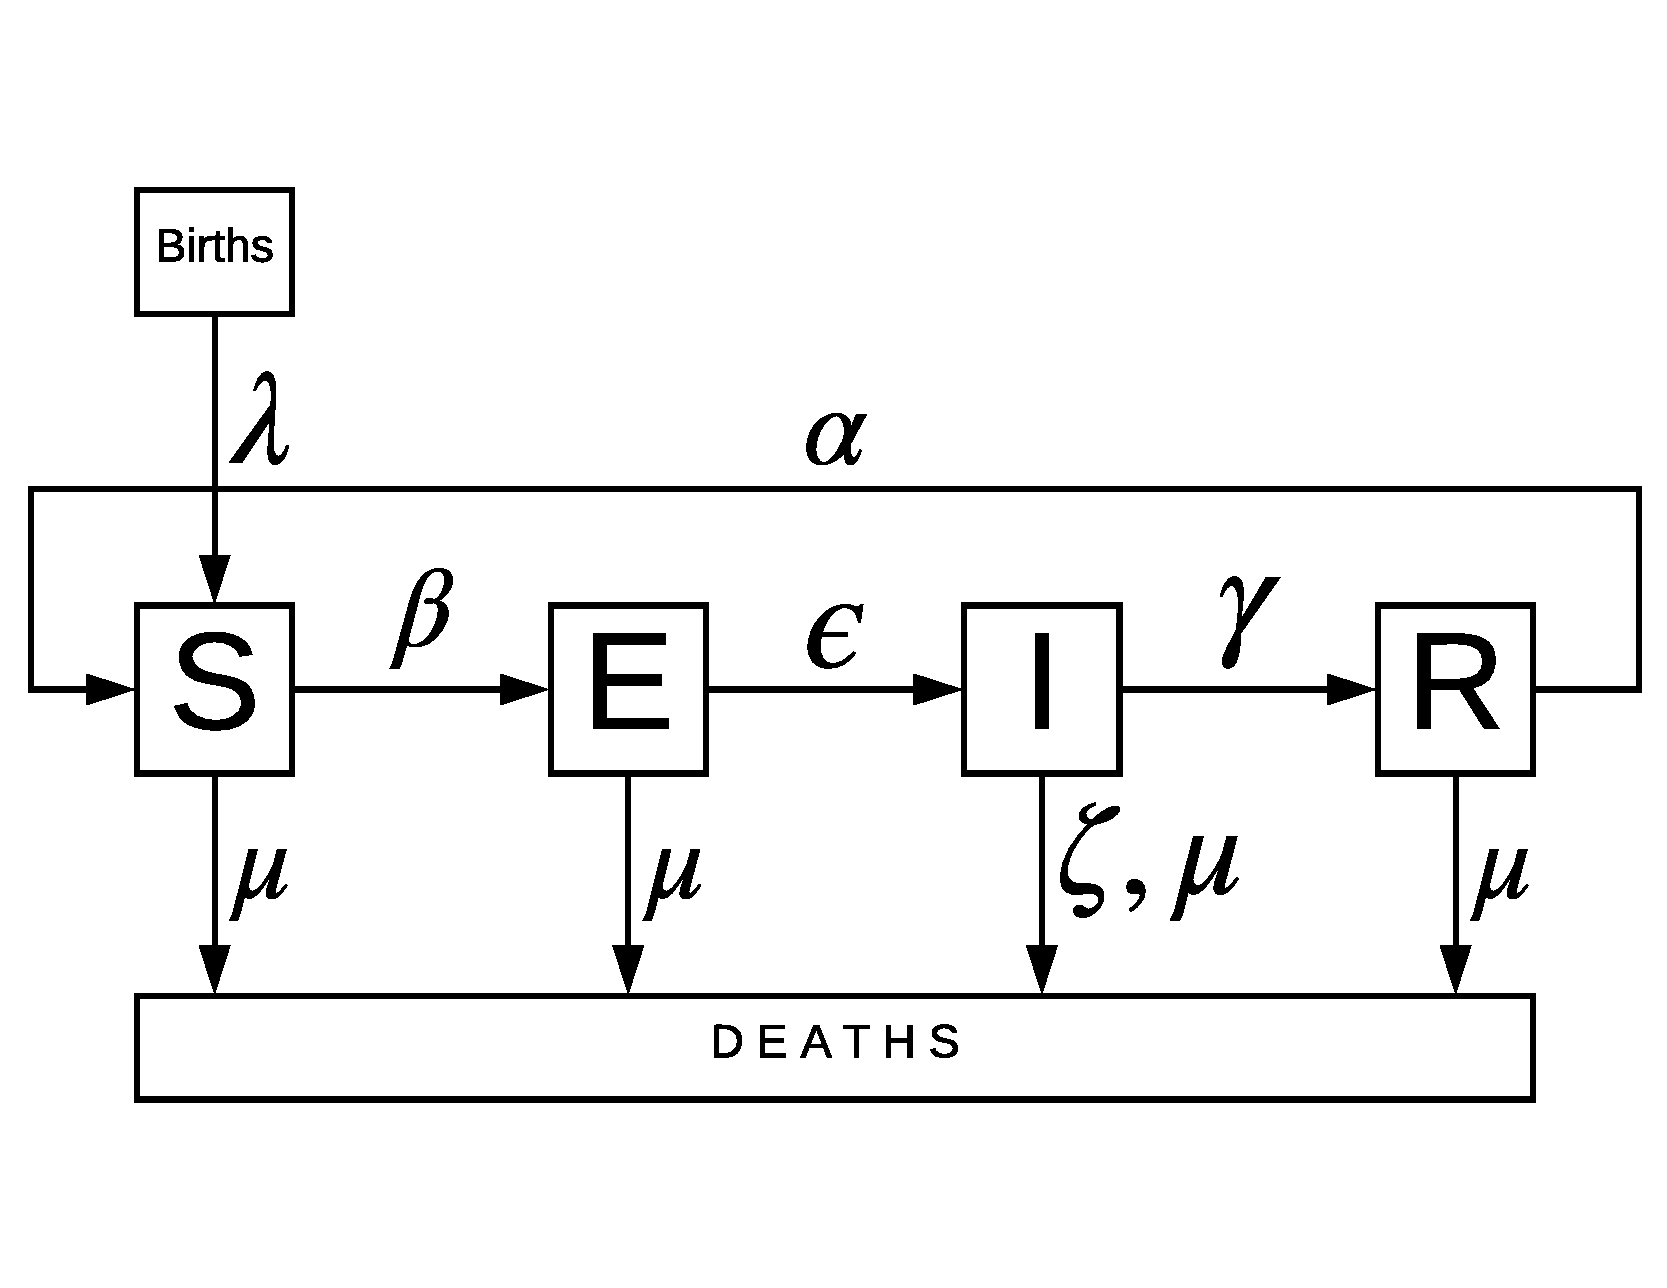
\includegraphics[scale=0.2]{lit_reviews/cs685_SEIR_model.pdf}
\end{column}
\begin{column}{0.48\textwidth}
\resizebox{0.65\columnwidth}{!}{
    \centering
    \begin{tabular}{|c l|}
    \hline
    Parameter & Description\\
    \hline
    $\lambda$ & Birth rate\\
    \hline
    $\mu$ & Death rate\\
    \hline
    $\beta$ & Transmission rate\\
    \hline
    $\epsilon$ & Incubation rate\\
    \hline
    $\gamma$ & Recovery rate\\
    \hline
    $\zeta$ & Infectious mortality rate\\
    \hline
    $\alpha$ & Immunity loss rate\\
    \hline
    \end{tabular}
}
\end{column}
\end{columns}
\end{frame}

%\begin{frame}{Example Formulation}
%    \begin{itemize}
%    \item A discrete-time model
%    \item[] \begin{align*}
%        p_{i}^{S}(t+1) &= \frac{R\alpha + \lambda N - \beta SI - \mu S}{N} = r\alpha + \lambda - (\beta i + \mu)s&\\
%        p_{i}^{E}(t+1) &= \frac{\beta SI - (\mu + \epsilon)E}{N} = \beta si - (\mu + \epsilon)e&\\
%        p_{i}^{I}(t+1) &= \frac{\epsilon E - (\mu + \gamma + \zeta)I}{N} = \epsilon e - (\mu + \gamma + \zeta)i&\\
%        p_{i}^{R}(t+1) &= \frac{\gamma I - (\mu + \alpha)R}{N} = \gamma i - (\mu + \alpha)r&\\
%        N &= s + e + i + r
%        p_{i}^{S}(t+1) &= f
%    \end{align*}
%    \item S,E,I,R,N: number of individuals in each compartment and whole population
%    \item s,e,i,r: relative fraction of individuals in each compartment (e.g. $r = \frac{R}{N}$)
%    \item All of the above are functions of $t$ except where noted
%   \end{itemize}
%\end{frame}

\begin{frame}{Example Formulation}
    \begin{itemize}
    \item[] \begin{align*}
    \frac{dS_{i}}{dt} &= \alpha R_{i} - \frac{\beta_{i} S_{i} I_{i}}{N_{i}} + \lambda N_{i} - \mu S_{i}\\
    \frac{dE_{i}}{dt} &= \frac{\beta_{i} S_{i} I_{i}}{N_{i}} - (\epsilon + \mu ) E_{i}\\
    \frac{dI_{i}}{dt} &= \epsilon E_{i} - (\gamma + \zeta + \mu)I_{i}\\
    \frac{dR_{i}}{dt} &= \gamma I_{i} - (\alpha + \mu)R_{i}\\
    \frac{dN_{i}}{dt} &= S_{i} + E_{i} + I_{i} + R_{i}
    \end{align*}
    \item Terms like $\epsilon E$ can be interpreted as exponentially-distributed waiting times with mean wait time $\frac{1}{\epsilon}$
   \end{itemize}
\end{frame}

\begin{frame}{Theoretical Work}
    \begin{itemize}
        \item Several important threshold values have been derived mathematically:
        \begin{itemize}
            \item $R_{0}$: Basic reproduction number - avg. number of infections for one infective and susceptible population
            \item $\sigma$: Contact number - avg. number of adequate contacts for one infective
            \item $R$: Replacement number - avg. number of secondary infections caused by each infective
        \end{itemize}
        \item Results in the field do not necessarily require simulations. Much has been done with "just the math"
        \item Approximation methods like mean-field theory are the norm
    \end{itemize}
\end{frame}

\begin{frame}{Agent-Based Simulations}
    \begin{itemize}
        \item Simulations that model each individual in the population have shown promise
        \item Models have many parameters and are usually not amenable to mathematical analysis
        \item Parameters can vary for each agent to capture the idea of different individuals
        \item These rely on averaging values measured over an ensemble of simulation to estimate parameters
        \item We ultimately chose an agent-based approach because it is simple to implement and describe while still providing good results
        \item It also fits well with the information diffusion model we chose
    \end{itemize}
\end{frame}

\begin{frame}{The Model for Viral Hoaxes}
\begin{itemize}
    \item A graph where each node is in one of three states:
    \begin{itemize}
        \item Believer
        \item Fact-checker
        \item Susceptible
    \end{itemize}
    \item Captures three phenomena:
    \begin{itemize}
        \item Spreading (based on neighbors)
        \item Verifying (fixed probability)
        \item Forgetting (fixed probability)
    \end{itemize}
\end{itemize}
%Briefly mention what mean field theory is and why it's important for this model
%Discuss the use of (1+a) and (1-a) instead of a and (1-a) in the spreading functions
%Prepare notes to show derivations or at least sketch them if needed
\end{frame}

\begin{frame}{Helpful Diagram}
    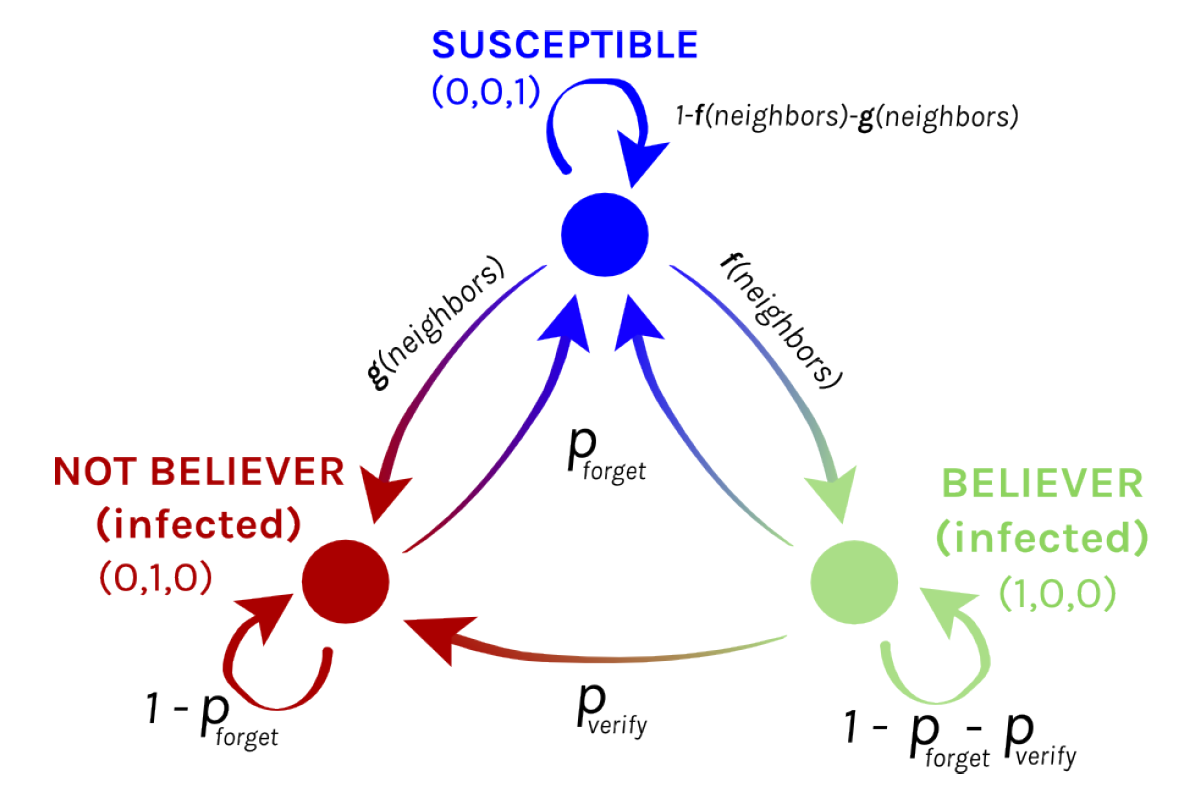
\includegraphics[width=\linewidth]{fig_1}
\end{frame}

\begin{frame}{The Spreading Functions}
    \begin{itemize}
        \item Capture how each node is affected by neighbors
        \item $f_{i}(t)$ and $g_{i}(t)$ represent spreading of the hoax and debunking respectively
        \begin{align*}
            f &= \beta \frac{n_{B}(1 + \alpha)}{n_{F}(1 - \alpha) + n_{B}(1 + \alpha)} \\
            g &= \beta \frac{n_{F}(1 - \alpha)}{n_{F}(1 - \alpha) + n_{B}(1 + \alpha)}
        \end{align*}
        \item Constants:
        \begin{itemize}
            \item $\alpha \in [0,1)$ credibility of hoax 
            \item $\beta \in [0,1)$ spreading probability
        \end{itemize}
        \item $n_{B},n_{F}$: number of adjacent believers, fact-checkers for node $i$ at time $t$
    \end{itemize}
\end{frame}
%\begin{frame}{A Simpler SEIR Model}
% 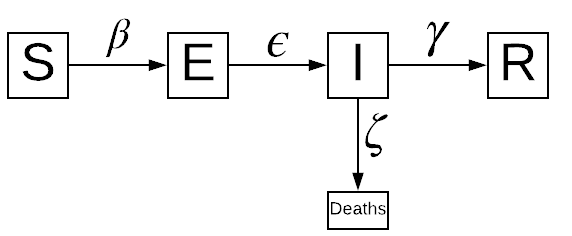
\includegraphics[width=\textwidth]{lit_reviews/cs685_SEIR_model_ours.png}
%\end{frame}
%\begin{frame}{Simplifications}
%\begin{itemize}
%    \item Ignore loss of immunity. Why: Modern measles vaccinations work long-term \cite{pinkbookMeasles}
%    \item Ignore births and deaths due to other causes. An measles epidemic occurs over a relatively short time
%\end{itemize}
%\end{frame}

\begin{frame}{Our Approach: Modelling Transmission (S-E)}
\begin{itemize}
    \item We discard assumption of random interactions
    \item Replace with a network where people are nodes and sufficient interactions are edges
    \item Interactions are cumulative - the graph represents all sufficient interactions per time step
    \item All nodes linked to a node in compartment I will have a 90\% chance to enter the "exposed" compartment
\end{itemize}
\end{frame}

\begin{frame}{Our Approach: Other Movements Between Compartments (E-I-R)}
\begin{itemize}
    \item Movement from E to I and from I to R occurs after randomly-selected time in compartment
    \item E-I: Incubation period is 10-12 days
    \item I-R: Transition when patient is no longer contagious. No longer considered contagious 4 days after onset of rash. 10-12 incubation, 1-2 prodrome, 5-6 rash, so 5-6 days total
    \item Death rate approximately 0.2\% from CDC surveillance data 1985-1992
\end{itemize}
\end{frame}

\begin{frame}{Formulation}
\begin{columns}
\begin{column}[t]{0.5\textwidth}
   \begin{align*}
      %p_{i}^{E}(t+1) &= \\
      p_{i}^{I}(t+1) &= \frac{\tau_{i}^{I}(t)}{X_{I}}\\
      p_{i}^{R}(t+1) &= \frac{\tau_{i}^{R}(t)}{X_{R}} + \zeta
   \end{align*}
   \renewcommand{\arraystretch}{1.3}
   %\begin{tabular}{C | C | C | C | C }
    %    \hphantom{ } & S & E & I & R\\
     %   \hline
      %  S & 1-p_{i}^{E} & p_{i}^{E} & 0 & 0\\
       % E & 0 & 1-p_{i}^{I} & p_{i}^{I} & 0\\
        %I & 0 & 0 & 1-p_{i}^{R} & p_{i}^{R}\\
        %R & 0 & 0 & 0 & 1\\
   %\end{tabular}
   \begin{tabular}{C | C | C | C }
        \hphantom{ } & E & I & R\\
        \hline
        E &  1-p_{i}^{I} & p_{i}^{I} & 0\\
        I &  0 & 1-p_{i}^{R} & p_{i}^{R}\\
        R &  0 & 0 & 1\\
   \end{tabular}
   \captionof*{table}{Transition Matrix}
\end{column}
\begin{column}[t]{0.5\textwidth}
\begin{itemize}
    \item $\tau_{i}^{E,I,R}(t)$: Length of time node $i$ has been in in compartment $E,I,R$
    \item $X_{E,I,R}$: Number of time steps node $i$ should remain in compartment $E,I,R$
    \item Value of $X_{E,I,R}$ is a realization of a normally-distributed random variable
    \item Infective individuals who die from the disease are considered recovered
\end{itemize}
\end{column}
\end{columns}
\end{frame}

\begin{frame}{Evaluation}
    \begin{itemize}
        \item Model as described is difficult to analyze mathematically
        \item Numerical results can be obtained by averaging an ensemble of simulations
        \item These could be compared with previous results e.g. for the basic reproduction number
        \item Epidemic model should be evaluated in isolation and with the information diffusion model
    \end{itemize}
\end{frame}
\end{document}